\section{Introdução}


Nesta etapa do projeto fiz testes com dois sensores acelerômetros:

MMA8452 e MPU6050

Como resultado optei por utilizar o sensor MPU6050 por sua grande variedade de bibliotecas,
baixo custo, 16 bits de resolução e, principalmente, por possuir sensor acelerômetro e giroscópio em um mesmo chip MEMS\footcite{MEMS: Micro Eletro Mechanical System.}.

O Microcontrador ESP32 e o sensor acelerômetro foram colados em uma pequena caixa onde futuramente pode ser adicionado uma bateria. Podemos ve-lo na Figura 1.


\begin{figure}[H]
    \center
    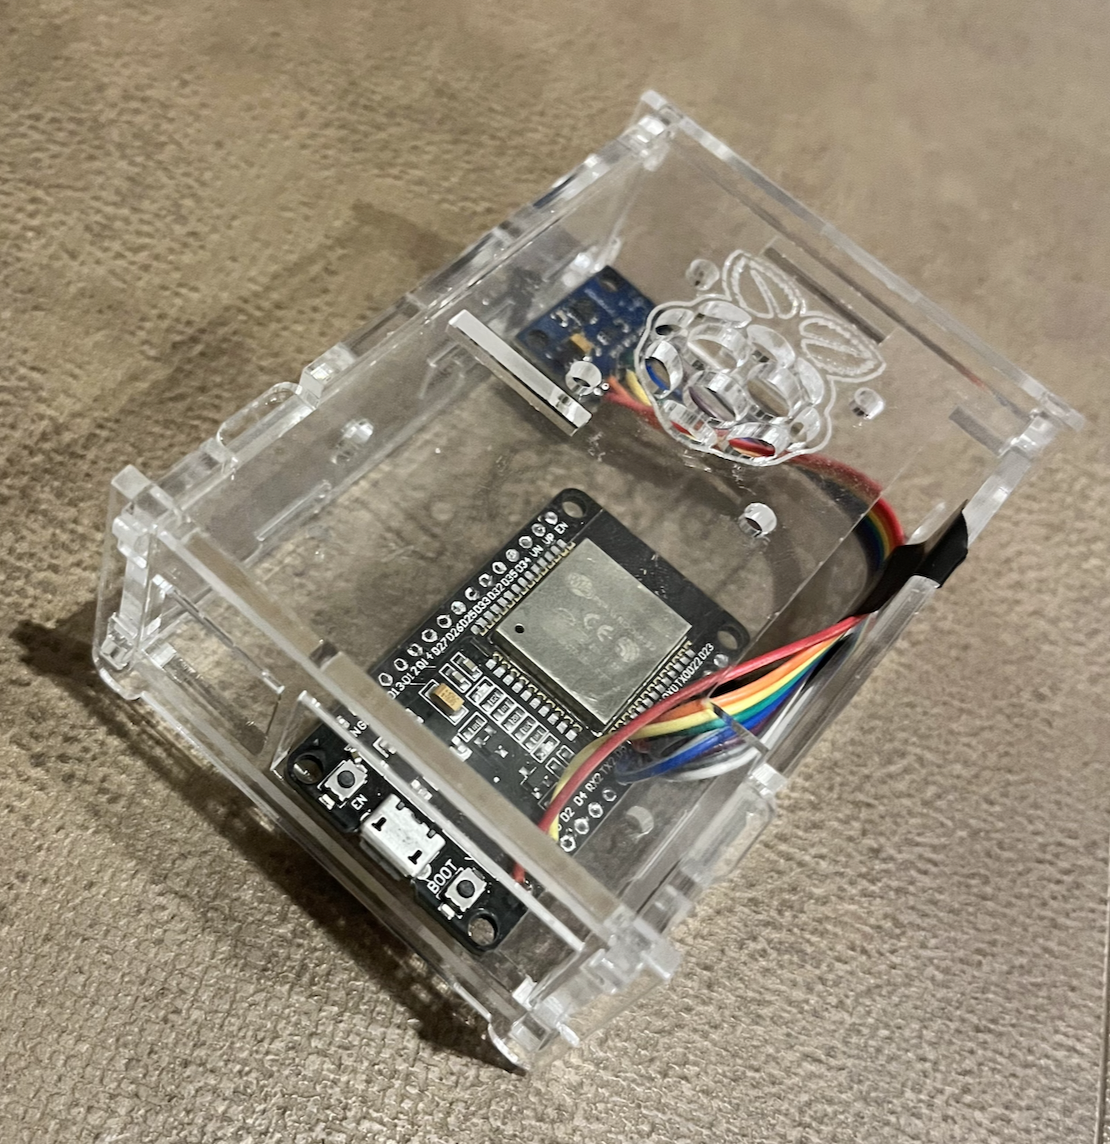
\includegraphics[width=6cm]{images/Prototipo}
    \caption{Prototipo}
\end{figure}
